\chapter{Lezione 7 - Workflow - Flusso lavorativo}

Benvenuti a tutti a questa lezione sul flusso lavorativo, workflow.
Gli argomenti che tratteremo in questa lezione sono due definizioni di flusso di lavoro, vedremo le caratteristiche di un sistema per la gestione automatica dei flussi di lavoro e analizzeremo l'architettura di un sistema per la gestione dei flussi di lavoro presentata dalla workflow management coalition.

Argomenti trattati:

\FloatBarrier
\begin{figure}[H]
  \centering
  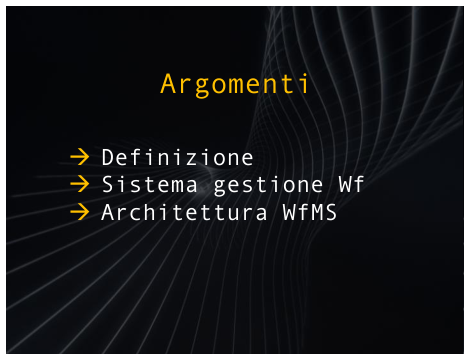
\includegraphics[width=0.50\textwidth,
                    trim=40 100 40 60, % L B R T
                    clip]
                    {images/Lez07_p01_fig_02}
  % \caption{Sommario}
  % \label{fig:Lez15_p06_fig_02}
\end{figure}
\FloatBarrier
\noindent

\FloatBarrier
\begin{figure}[H]
  \centering
  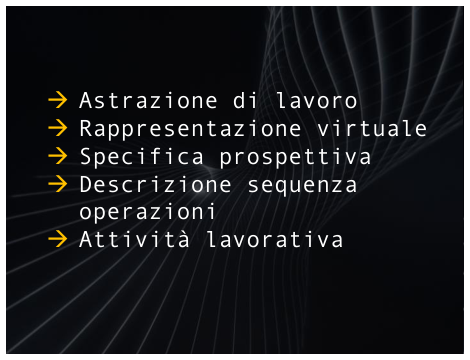
\includegraphics[width=0.50\textwidth,
                    trim=40 100 20 60, % L B R T
                    clip]
                    {images/Lez07_p01_fig_04}
  % \caption{Sommario}
  % \label{fig:Lez15_p06_fig_02}
\end{figure}
\FloatBarrier
\noindent

Vediamo la prima definizione, una definizione consolidata, una definizione d'uso che considera un workflow una astrazione di un'attività lavorativa, una sua rappresentazione virtuale, siamo nel digitale, quindi dobbiamo formalizzare e descrivere il modello dell'attività lavorativa in termini leggibili e interpretabili da un calcolatore.

La rappresentazione del flusso di lavoro è fatta, progettata, concepita secondo una specifica prospettiva, vedremo che abbiamo cinque prospettive differenti per vedere il flusso di lavoro a seconda delle caratteristiche e degli elementi costituenti su cui vorremo focalizzare l'attenzione.

Un workflow è una descrizione di una sequenza di operazioni svolte da individui, da un gruppo, da organizzazioni, operazioni semplici interrelate ed eventualmente aggregate in operazioni più complesse.

Il flusso di lavoro, un workflow, quindi descrive un'attività lavorativa composta di attività elementari connesse, svolte, eseguite in una sequenza specificata, non esistono attese tra l'esecuzione di un'attività e l'altra e ogni task viene concluso, ogni attività elementare viene conclusa prima dell'inizio della seguente.

\FloatBarrier
\begin{figure}[H]
  \centering
  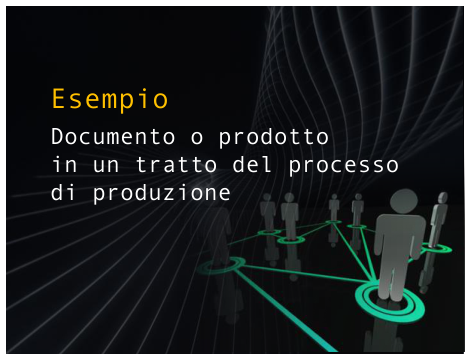
\includegraphics[width=0.50\textwidth,
                    trim=40 100 20 60, % L B R T
                    clip]
                    {images/Lez07_p01_fig_05}
  % \caption{Sommario}
  % \label{fig:Lez15_p06_fig_02}
\end{figure}
\FloatBarrier
\noindent

Come esempio possiamo considerare il processo di produzione di un documento in un tratto del suo ciclo di vita o anche semplicemente la sequenza di attività che permettono di crearlo, di modificarlo, di verificare la versione, di accettare una versione, di passarla alla pubblicazione per la sua diffusione e cominciarne la diffusione.

Le descrizioni delle singole attività comportano l'accompagnamento con le risorse che vengono utilizzate e i differenti attori che svolgono i ruoli previsti dalle differenti attività.

\FloatBarrier
\begin{figure}[H]
  \centering
  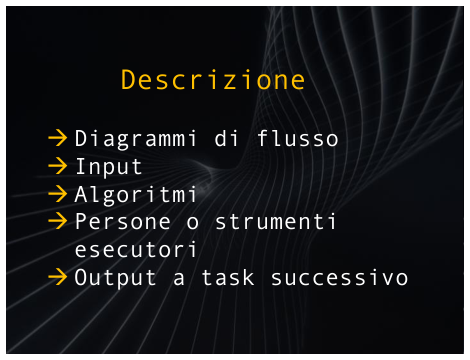
\includegraphics[width=0.50\textwidth,
                    trim=40 60 20 60, % L B R T
                    clip]
                    {images/Lez07_p01_fig_06}
  % \caption{Sommario}
  % \label{fig:Lez15_p06_fig_02}
\end{figure}
\FloatBarrier
\noindent

Un workflow viene descritto materialmente mediante dei diagrammi di flusso, quindi devono essere mostrati gli input, e gli input possono essere informazione, nel caso stiamo descrivendo come nell'esempio precedente la costituzione di un documento, un processo di elaborazione di informazione, ma possiamo anche considerare un workflow di una produzione materiale, quindi di un manufatto o un'elaborazione di energia.

I flussi di lavoro rendono conto delle attività descritte mediante algoritmi, mediante processi automatizzati, con la specifica delle persone o degli strumenti che intervengono nella realizzazione, nella esecuzione.

\FloatBarrier
\begin{figure}[H]
  \centering
  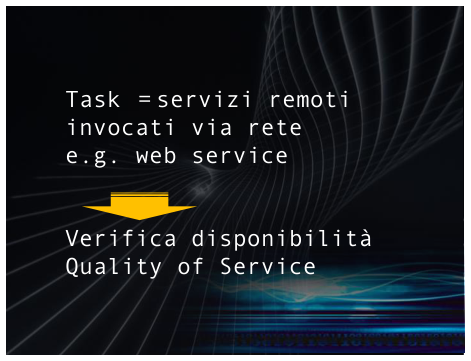
\includegraphics[width=0.50\textwidth,
                    trim=40 60 20 60, % L B R T
                    clip]
                    {images/Lez07_p02_fig_01}
  % \caption{Sommario}
  % \label{fig:Lez15_p06_fig_02}
\end{figure}
\FloatBarrier
\noindent

Ogni output viene prodotto e passato al task successivo per la sua attivazione.
I task di un workflow, le singole azioni elementari possono essere svolte localmente nel sistema automatico di supporto, ma possono anche essere task remoti, quindi task svolti da postazione lontanea localizzate, in questo caso saranno postazioni collegate via rete che permettono l'invocazione di questi servizi, per esempio attraverso l'uso di web services, che sono un tipo di interfaccia che permette di esporre delle modalità di richiesta dei servizi e permettere così lo sviluppo di applicazioni eventualmente remote, sviluppate in maniera concorrente al sistema centrale che stiamo utilizzando e ne permettono l'accesso.

Questo però richiede una verifica di quali sono i servizi disponibili e questo viene fatto tramite dei cataloghi, delle disponibilità quindi delle funzionalità che sono offerte all'accesso remoto e la qualità del servizio.

Nella gestione di servizi offerti in maniera localizzata è importante la stabilità della connessione e l'efficacia e l'efficienza del servizio stesso.

\FloatBarrier
\begin{figure}[H]
  \centering
  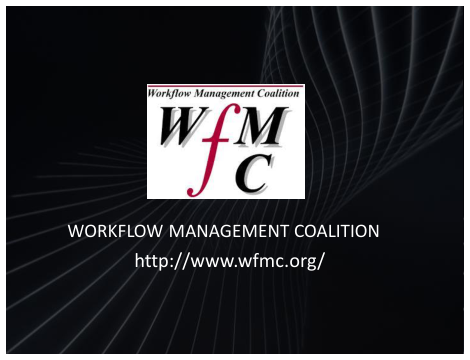
\includegraphics[width=0.50\textwidth,
                    trim=40 60 20 60, % L B R T
                    clip]
                    {images/Lez07_p02_fig_02}
  % \caption{Sommario}
  % \label{fig:Lez15_p06_fig_02}
\end{figure}
\FloatBarrier
\noindent

Vediamo ora una definizione proposta dalla workflow management coalition.
Warflow management coalition è un consorzio costituito nel maggio del 1993 da alcuni partner commerciali quali la Black Forest Group, l'IBM, la Hewlett Packard, la Fujitsu, la ICL e 300 tra software e service houses.
E' un consorzio, orientato alla definizione di norme per l'interoperabilità tra i sistemi di workflow management.
Non necessariamente quindi la certificazione dei servizi, la valutazione dei servizi ma orientata alla definizione delle norme che devono essere rispettate.


\FloatBarrier
\begin{figure}[H]
  \centering
  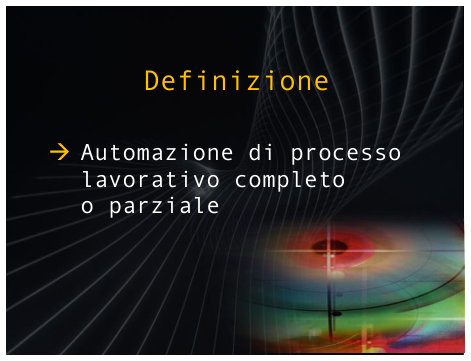
\includegraphics[width=0.50\textwidth,
                    trim=40 120 40 60, % L B R T
                    clip]
                    {images/Lez07_p02_fig_03}
  % \caption{Sommario}
  % \label{fig:Lez15_p06_fig_02}
\end{figure}
\FloatBarrier
\noindent


La definizione proposta: il workflow è l'automazione di un processo lavorativo completo o parziale.

Perché prevediamo la possibilità che sia automatizzato il processo complessivamente o parzialmente?

Perché il processo può essere molto complesso, il processo può richiedere strumenti anche differenti per un'automazione di tratti del percorso lavorativo differenti, quindi parcellizzato per poterlo trattare in maniera più analitica.

\FloatBarrier
\begin{figure}[H]
  \centering
  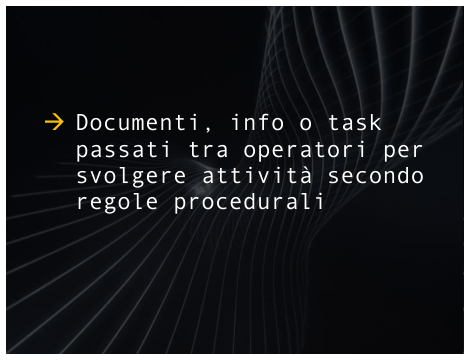
\includegraphics[width=0.50\textwidth,
                    trim=40 100 20 60, % L B R T
                    clip]
                    {images/Lez07_p02_fig_04}
  % \caption{Sommario}
  % \label{fig:Lez15_p06_fig_02}
\end{figure}
\FloatBarrier
\noindent

Il workflow richiede il trattamento dei documenti, delle informazioni e delle attività task, quindi parliamo delle attività elementari che vengono svolte e dei documenti e delle informazioni che sono passate tra gli operatori per svolgere attività secondo le regole procedurali, i protocolli.

Quindi il workflow rende conto anche delle informazioni di processo, che sono prodotte durante le attività, le informazioni che vengono prodotte come risultati dei singoli task, la documentazione di supporto per queste informazioni e per le attività svolte, ma anche le informazioni di controllo all'intero processo.

Vi propongo ora due spunti di riflessione, provate a proporre, a concepire un processo di lavoro e descrivetene graficamente il diagramma di flusso che lo rappresenta.

\section{Sistema per la gestione dei WF}

\FloatBarrier
\begin{figure}[H]
  \centering
  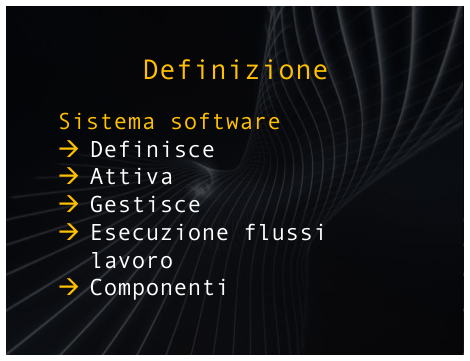
\includegraphics[width=0.50\textwidth,
                    trim=40 40 20 40, % L B R T
                    clip]
                    {images/Lez07_p03_fig_01}
  % \caption{Sommario}
  % \label{fig:Lez15_p06_fig_02}
\end{figure}
\FloatBarrier
\noindent

Vediamo ora la definizione di un sistema per la gestione di workflow.
È un sistema software che permette la definizione, l'attivazione, la gestione e l'esecuzione di flussi di lavoro, quindi deve disporre di componenti quali un workflow engine, quindi un'interprete delle descrizioni o dei flowcharts che sono stati utilizzati per descrivere il flusso di lavoro, un'interprete delle definizioni prodotte, un ambiente per produrre queste definizioni, quindi specificare le risorse, gli attori e darne una descrizione interpretabile dal workflow engine, un'interfaccia agevole che permette il controllo e l'esecuzione, la visualizzazione delle varie fasi del processo lavorativo e possibilmente un interoperabile interfacciamento con strumenti ICT o interni all'organizzazione ma sviluppati indipendentemente o esterni, richiamati  attraverso eventualmente un interfacciamento tipo web services.

\subsection{Workflow engine}

\FloatBarrier
\begin{figure}[H]
  \centering
  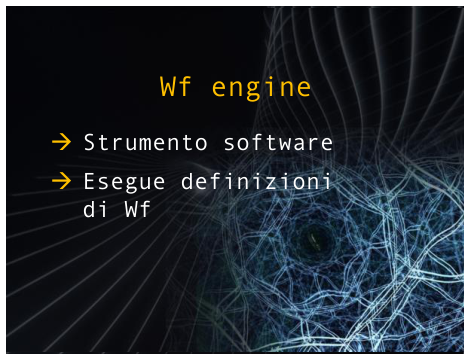
\includegraphics[width=0.50\textwidth,
                    trim=40 100 20 60, % L B R T
                    clip]
                    {images/Lez07_p03_fig_02}
  % \caption{Sommario}
  % \label{fig:Lez15_p06_fig_02}
\end{figure}
\FloatBarrier
\noindent


Il workflow engine abbiamo visto è uno strumento software che esegue le descrizioni che sono state prodotte, le definizioni che sono state prodotte per un workflow.

\FloatBarrier
\begin{figure}[H]
  \centering
  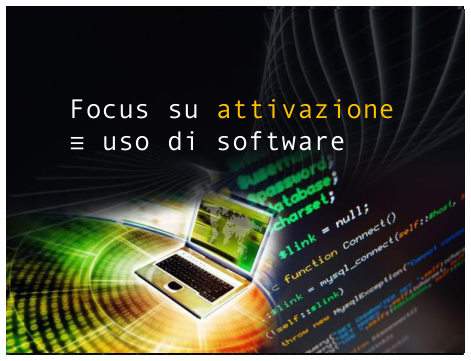
\includegraphics[width=0.50\textwidth,
                    trim=40 160 20 60, % L B R T
                    clip]
                    {images/Lez07_p03_fig_03}
  % \caption{Sommario}
  % \label{fig:Lez15_p06_fig_02}
\end{figure}
\FloatBarrier
\noindent

Fatemi notare che il focus sull'attivazione corrisponde al considerare un flusso di lavoro, un workflow, come un elemento eseguibile da un software, un elemento di software.

Stiamo dicendo che le descrizioni di cui noi stiamo parlando di un flusso di lavoro sono descrizioni di un'astrazione di un flusso di lavoro reale, di un flusso di lavoro effettivamente svolto e sono descrizioni eseguibili da un calcolatore, quindi verranno effettuate da linguaggi particolari.

\subsection{Strumenti ICT a supporto del workflow management}

Ma vediamo adesso ci sono quattro categorie di strumenti ICT a supporto del workflow management.

\FloatBarrier
\begin{figure}[H]
  \centering
  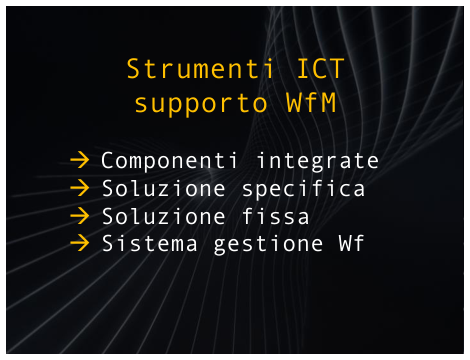
\includegraphics[width=0.50\textwidth,
                    trim=40 40 20 40, % L B R T
                    clip]
                    {images/Lez07_p03_fig_04}
  % \caption{Sommario}
  % \label{fig:Lez15_p06_fig_02}
\end{figure}
\FloatBarrier
\noindent

Le componenti integrate, le componenti integrate si rivolgono a sistemi integrati in sistemi più complessi, moduli per il workflow management che vengono integrati in sistemi aziendali più complessi, oppure soluzioni specifiche rivolte a specifiche imprese per la gestione di più casi di processi lavorativi richiesti al loro interno, ma non per una gestione generale.

Il caso successivo, la classe successiva, le soluzioni fisse si rivolgono invece a casi fissati la cui descrizione è esplicitata nell'applicativo, non viene quindi fornito supporto generale, una qualunque modifica alla descrizione di questo caso richiede l'intervento sull'applicativo, quindi non è prevista una coreografia.

Per coreografia intendiamo la definizione degli elementi di elaborazione, quindi dei moduli che costituiscono un sistema e delle loro interrelazioni sia per il flusso informativo sia per il tipo di comunicazione.
E' lo stabilire le regole generali che devono essere rispettate per l'orchestrazione.

Quindi la base per la successiva categoria di strumenti ict a supporto dei workflow, i sistemi di gestione dei workflow generali che permettono, vedremo nel seguito, tutte le funzionalità per la definizione, l'esecuzione, la gestione e l'estensione dei flussi di lavoro.

\subsection{Orchestrazione}

Ma è bene spendere due parole sulla orchestrazione che è un'attività realizzativa di progettazione e di implementazione rilevante per questo tipo di sistemi.

\FloatBarrier
\begin{figure}[H]
  \centering
  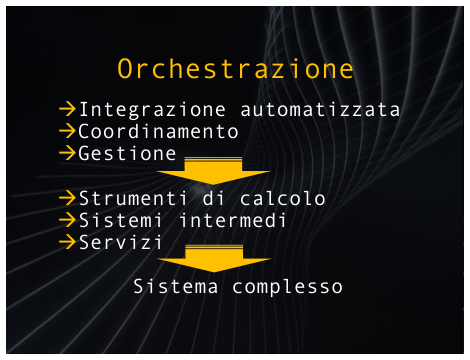
\includegraphics[width=0.50\textwidth,
                    trim=40 40 20 40, % L B R T
                    clip]
                    {images/Lez07_p03_fig_05}
  % \caption{Sommario}
  % \label{fig:Lez15_p06_fig_02}
\end{figure}
\FloatBarrier
\noindent

L'orchestrazione è l'integrazione automatizzata, il coordinamento e la gestione di strumenti di calcolo che vengono integrati e gestiti attraverso l'utilizzo di sistemi intermedi, back-end, che effettuano l'orchestrazione dei diversi attori automatici che intervengono per l'offerta di servizi.
L'attività orchestrata, l'attività svolta da ogni elemento, da ogni attore che viene orchestrato, secondo le regole definite nella coreografia, svolge un servizio.
In questo modo sono costituiti sistemi complessi integrati.

\FloatBarrier
\begin{figure}[H]
  \centering
  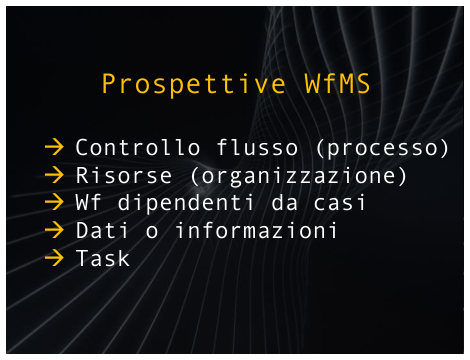
\includegraphics[width=0.50\textwidth,
                    trim=40 40 20 40, % L B R T
                    clip]
                    {images/Lez07_p03_fig_06}
  % \caption{Sommario}
  % \label{fig:Lez15_p06_fig_02}
\end{figure}
\FloatBarrier
\noindent

Ma vediamo ora che esistono cinque prospettive da cui possiamo osservare e analizzare i sistemi per la gestione dei flussi di lavoro.

Una prospettiva di processo, la prospettiva controllo di flusso, una prospettiva che focalizza sulle risorse, quindi una prospettiva di organizzazione, i casi, quindi workflow che dipendono dai casi, i dati o le informazioni che abbiamo visto precedentemente possono essere procedurali, quindi prodotti dalle fasi di lavoro o di controllo, quindi per il corretto svolgimento della completa attività lavorativa e da ultimo la focalizzazione sulle singole attività.

Ma vediamo la prima prospettiva, la prospettiva relativa al controllo del flusso.

\FloatBarrier
\begin{figure}[H]
  \centering
  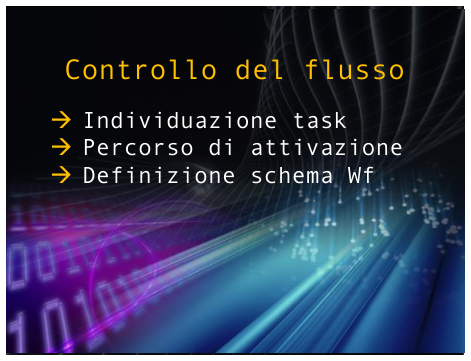
\includegraphics[width=0.50\textwidth,
                    trim=40 120 20 40, % L B R T
                    clip]
                    {images/Lez07_p04_fig_01}
  % \caption{Sommario}
  % \label{fig:Lez15_p06_fig_02}
\end{figure}
\FloatBarrier
\noindent

Richiede l'individuazione delle singole attività e la definizione del percorso di attivazione.

Il percorso che può essere definito sequenziale, quindi ogni task viene eseguito successivamente all'altro ordinatamente, oppure condizionato, quindi alcuni task possono essere previsti nella descrizione del flusso di lavoro ma eseguiti solo sotto determinate situazioni.

L'esecuzione di task può essere parallela, concorrente, quindi svolta contemporaneamente nel tempo, oppure ciclica, quindi possiamo descrivere un flusso di lavoro con dei task che vengono ripetute.
Indicheremo quindi con una struttura di controllo le volte che dovremo ripetere questo sottopercorso, questo sottoprocesso del flusso di lavoro.

Infine dovremo disporre di funzionalità per la definizione dello schema complessivo del processo lavorativo.

\FloatBarrier
\begin{figure}[H]
  \centering
  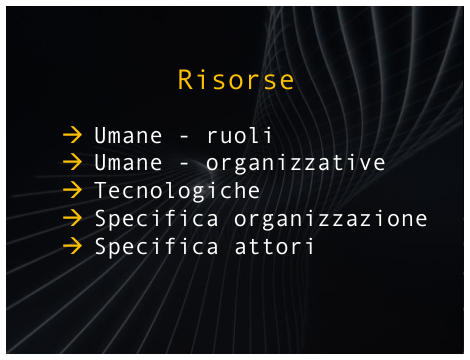
\includegraphics[width=0.50\textwidth,
                    trim=40 80 20 60, % L B R T
                    clip]
                    {images/Lez07_p04_fig_02}
  % \caption{Sommario}
  % \label{fig:Lez15_p06_fig_02}
\end{figure}
\FloatBarrier
\noindent

Nella successiva prospettiva definiamo le risorse, specificatamente gli individui con i ruoli, i gruppi dovremo definire le loro relazioni e le risorse effettivamente che vengono a loro allocate, a loro assegnate.
Quindi vediamo la prospettiva delle risorse.

Sono definiti i ruoli specifici individualmente, quindi le singole persone come svolgono il loro lavoro, i task loro assegnati e con quali autorità, con quali autorizzazioni, con quali diritti di accesso al sistema, all'ambiente lavorativo.

In seguito sono definite le risorse organizzative, i gruppi, le comunità che lavorano collaborativamente nell'ambito dell'organizzazione per svolgimento dei task loro assegnati.

Sono definite poi le risorse tecnologiche, ora non con i ruoli assegnati, ma con lo svolgimento delle attività, con la finalità a cui sono destinati nell'ambito del workflow.

A questo punto dobbiamo definire le relazioni tra i vari gruppi, i vari individui nell'ambito dell'organizzazione e, infine, la specifica degli attori con le assegnate risorse umane o tecnologiche o le relazioni individui-gruppi.

\FloatBarrier
\begin{figure}[H]
  \centering
  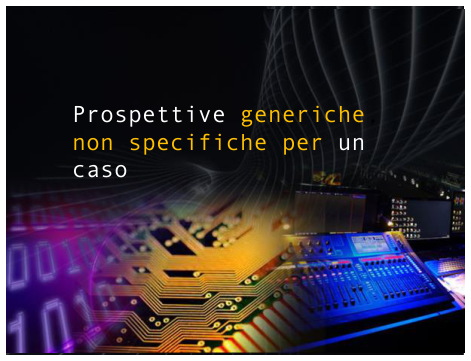
\includegraphics[width=0.50\textwidth,
                    trim=40 120 20 60, % L B R T
                    clip]
                    {images/Lez07_p04_fig_03}
  % \caption{Sommario}
  % \label{fig:Lez15_p06_fig_02}
\end{figure}
\FloatBarrier
\noindent

Quindi costruiamo la rete organizzativa.
Le prospettive sono generiche, non specifiche, per un caso.

\FloatBarrier
\begin{figure}[H]
  \centering
  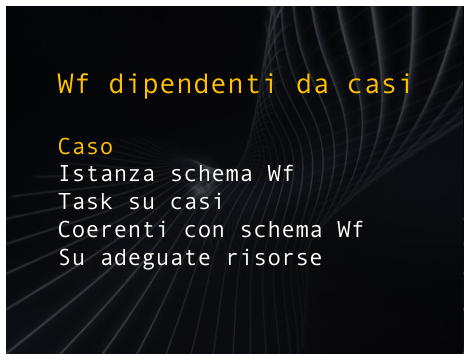
\includegraphics[width=0.50\textwidth,
                    trim=40 80 20 60, % L B R T
                    clip]
                    {images/Lez07_p04_fig_04}
  % \caption{Sommario}
  % \label{fig:Lez15_p06_fig_02}
\end{figure}
\FloatBarrier
\noindent

Vediamo quindi la prospettiva dipendente dai casi.
Cos'è un caso?
Un caso è un'istanza di schema di flusso di lavoro, i task sono definiti sui casi in questa prospettiva, quindi su situazioni pratiche, sono coerenti però con lo schema del workflow e effettuati, eseguiti sulle adeguate risorse assegnate.

\FloatBarrier
\begin{figure}[H]
  \centering
  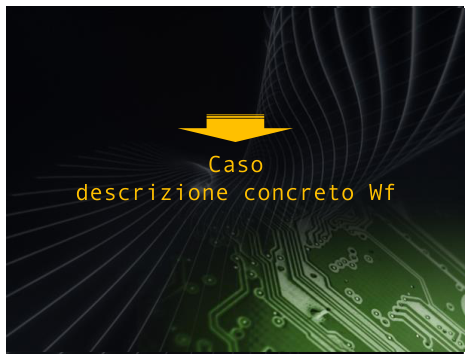
\includegraphics[width=0.50\textwidth,
                    trim=40 120 20 100, % L B R T
                    clip]
                    {images/Lez07_p04_fig_05}
  % \caption{Sommario}
  % \label{fig:Lez15_p06_fig_02}
\end{figure}
\FloatBarrier
\noindent

Un caso è quindi una descrizione di un concreto, un reale flusso di lavoro.

\FloatBarrier
\begin{figure}[H]
  \centering
  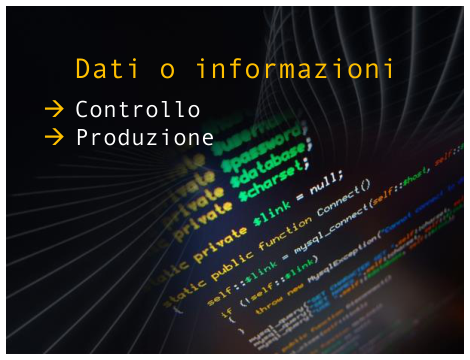
\includegraphics[width=0.50\textwidth,
                    trim=40 160 20 40, % L B R T
                    clip]
                    {images/Lez07_p04_fig_06}
  % \caption{Sommario}
  % \label{fig:Lez15_p06_fig_02}
\end{figure}
\FloatBarrier
\noindent

Passiamo alla prospettiva 4 riguardante i dati o le informazioni.
Abbiamo accennato precedentemente che abbiamo due tipi di dati o informazioni e di documentazione.
Per il controllo del processo di produzione del flusso di lavoro.

La seconda è per la produzione, quindi facciamo riferimento a dati, informazioni e documenti che vengono prodotti nel corso dei singoli task.

\FloatBarrier
\begin{figure}[H]
  \centering
  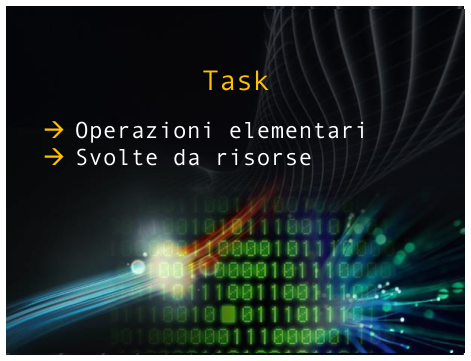
\includegraphics[width=0.50\textwidth,
                    trim=40 160 20 40, % L B R T
                    clip]
                    {images/Lez07_p05_fig_01}
  % \caption{Sommario}
  % \label{fig:Lez15_p06_fig_02}
\end{figure}
\FloatBarrier
\noindent

L'ultima prospettiva è la prospettiva dei task, le operazioni elementari che sono svolte in relazione alle risorse, quindi in questa prospettiva il fuoco sarà sulle attività elementari e sul controllo dell'uso e la disponibilità delle risorse.
Vediamo alcuni esempi di contesti in cui vi invito a definire alcuni flussi di lavoro quanto più complessi riuscite.

\FloatBarrier
\begin{figure}[H]
  \centering
  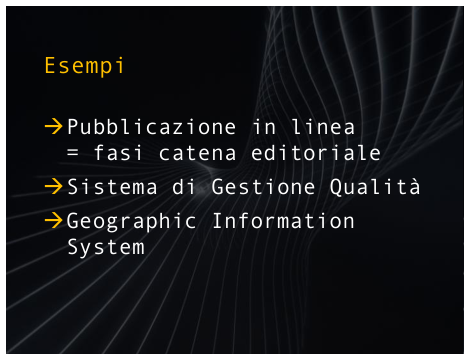
\includegraphics[width=0.50\textwidth,
                    trim=40 100 20 40, % L B R T
                    clip]
                    {images/Lez07_p05_fig_02}
  % \caption{Sommario}
  % \label{fig:Lez15_p06_fig_02}
\end{figure}
\FloatBarrier
\noindent

La pubblicazione in linea, le fasi della definizione della catena editoriale, dalla produzione, dall'editing di un documento fino alla sua diffusione sui canali di rete.

Un secondo contesto, un sistema di gestione della qualità.

Il sistema di gestione della qualità definisce per una specifica attività in un'organizzazione le regole, la modulistica, la documentazione che deve essere prodotta e la procedura che deve essere seguita, sostanzialmente la coreografia della attività in quel settore.

Altro contesto, il geographic information system.

Nell'ambito dei sistemi informativi territoriali sono tante le informazioni che vengono prodotte, che vengono acquisite, vengono acquisite da diverse sorgenti, diversi gruppi o dipartimenti che le producono, vengono assemblate e confezionate in modi differenti.

\FloatBarrier
\begin{figure}[H]
  \centering
  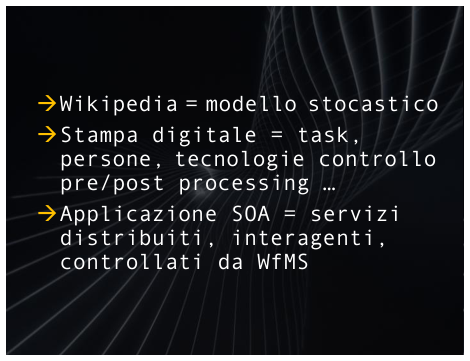
\includegraphics[width=0.50\textwidth,
                    trim=40 60 20 60, % L B R T
                    clip]
                    {images/Lez07_p05_fig_03}
  % \caption{Sommario}
  % \label{fig:Lez15_p06_fig_02}
\end{figure}
\FloatBarrier
\noindent

Possiamo riprendere la Wikipedia che ha un modello stocastico di organizzazione, di contribuzione e di valutazione.
Bisogna in questo caso analizzare, verificare il modo di lavoro e definire per una specifica attività, che sia una discussione, che sia l'editing di una pagina, che sia l'intero processo di produzione di un elemento di conoscenza, il flusso delle attività.

In seguito la stampa digitale, quindi task, le persone, le tecnologie che servono per il controllo pre e post processing prima e dopo la produzione e la successiva elaborazione del documento.

Un caso più tecnologico riguarda il service oriented architecture, services distributed, interagenti, controllati da un workflow management system che contribuiscono alla descrizione e produzione di attività viste come servizi offerti, servizi complessi, strutturati.

Vediamo ora uno spunto di riflessione.

Dettagliate l'esempio che avete proposto precedente con task, risorse umane, materiali, controllo e strumenti tecnologici di supporto.
Posso anche invitarvi a ridefinire anche il workflow, riprodurre la sua descrizione in uno dei contesti che abbiamo visto nel precedente catalogo lista di contesti lavorativi.

\subsection{Architettura dei WfMS}

\FloatBarrier
\begin{figure}[H]
  \centering
  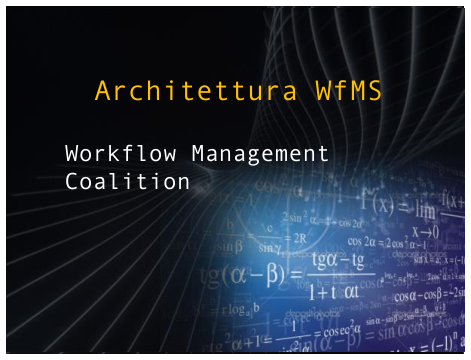
\includegraphics[width=0.50\textwidth,
                    trim=40 160 20 60, % L B R T
                    clip]
                    {images/Lez07_p05_fig_05}
  % \caption{Sommario}
  % \label{fig:Lez15_p06_fig_02}
\end{figure}
\FloatBarrier
\noindent

Passiamo ora all'architettura dei workflow management system.
Vedremo adesso l'architettura proposta, l'architettura di riferimento proposta dal workflow management coalition.

\FloatBarrier
\begin{figure}[H]
  \centering
  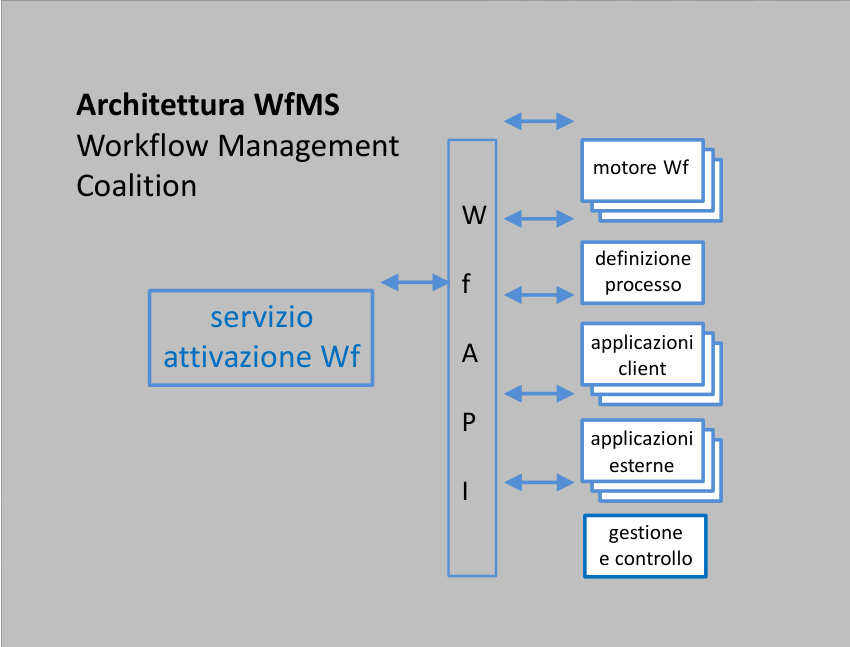
\includegraphics[width=0.50\textwidth,
                    trim=40 40 60 40, % L B R T
                    clip]
                    {images/Lez07_p05_fig_06}
  % \caption{Sommario}
  % \label{fig:Lez15_p06_fig_02}
\end{figure}
\FloatBarrier
\noindent

Vediamo quindi lo schema con le sue componenti.

Innanzitutto il servizio di attivazione del workflow.
È un ambiente che permette l'amministrazione, l'attivazione e il controllo di tutti gli elementi.
È l'ambiente di administration, l'ambiente del supervisore che attiva e controlla le varie fasi del processo di lavoro gestito dal sistema.

Poi abbiamo in sequenza logica l'elemento, il componente per la definizione del processo.

Questo componente deve fornire ambiente per la definizione del workflow, quindi la descrizione dei task, eventualmente descrivendo l'algoritmo dell'attività che devono svolgere, le risorse umane individuali e di gruppo, le risorse tecnologiche, quelle organizzative, quindi le relazioni tra gli elementi precedenti e l'assegnazione rispettiva delle varie risorse per svolgere il lavoro.

Queste descrizioni, abbiamo visto, sono descrizioni eseguibili da un calcolatore.
Devono essere eseguite dall'elemento, dal componente chiamato motore del workflow.
Questo componente altro non è che un interprete delle descrizioni automatiche prodotte del workflow.
Permetterà l'attivazione e il progresso.

Vi sono poi, vediamo, degli elementi indicati come applicazioni client.
Sono applicazioni prodotte all'interno dell'organizzazione, nuove, che possono interfacciarsi con le altre componenti, che possono svolgere delle attività coerenti con le altre componenti del nostro sistema per la gestione dei workflow, ma componenti sviluppate in tempi differenti.
Quindi sarà necessario un occhio d'attenzione all'interoperabilità.
Dopo vedremo da chi è gestita.

Il successivo componente indicato applicazioni esterne fa riferimento agli applicativi sviluppati da organizzazioni esterne alla nostra di riferimento, alla proprietaria, all'utente del sistema che stiamo descrivendo, a cui però è concesso il collegamento al nostro sistema o fa riferimento ad applicazioni che vengono sviluppate dall'esterno, quindi in tempi differenti, in situazioni differenti dalla realizzazione del nostro sistema e che vengono fornite all'organizzazione.
A maggior ragione sarà necessario fornire un opportuno sistema di interfacciamento e gestione dell'interoperabilità fra i diversi componenti del sistema interni ed esterni, nativi, applicazioni sviluppati client, quindi all'interno della nostra organizzazione, ma in tempi successivi, e applicazioni sviluppati da enti esterni.

L'ultimo elemento, il componente di gestione e controllo che serve per individuare, per controllare innanzitutto lo svolgimento dei singoli task, il flusso delle informazioni, individuare eventuali colli di bottiglia per permettere un efficace e un efficiente svolgimento delle attività e individuazione di eventuali vie di fuga che possano inficiare l'efficienza dello svolgimento delle attività.

L'interoperabilità comunicazionale e l'interoperabilità semantica quindi che ci permetta di fare riferimento a tutti i componenti con gli stessi significati assegnati alle informazioni è il workflow advanced programmi interface, che è l'interfaccia di programmazione offerta ai vari sviluppatori per collegare le varie componenti e permettere tra loro una corretta armonica comunicazione.

A questo punto vorrei offrirvi uno spunto di riflessione conclusivo di questo argomento e quindi della lezione.
Immaginate l'attivazione dei componenti dell'architettura di sistema proposta dalla workflow management coalition per produrre l'esempio precedente.

Quindi operate una sorta di simulazione con la descrizione di workflow che avete costruito e provate a vedere l'attivazione dei vari elementi durante lo svolgimento del vostro workflow.